%************************************************
\chapter{Comportamento termico}\label{chp:ComportamentoTermico}
%************************************************
Per andare ad analizzare il comportamento termico di un materiale polimerico consideriamo uno completamente amorfo, per il momento. 
Alla figura \ref{fig:Tg}, viene rappresentato il suo comportamento termico.
\graffito{All'aumentare della temperatura, dopo la transizione vetrosa, il materiale abbasserà ulteriormente il suo modulo elastico fino ad arrivare alla condizione di fluido ad alta viscosità}
Dal grafico si rilevano due zone separate dalla temperatura di transizione vetrosa $T_g$.
La prima zona si chiama di \textbf{vetro} ed è la zona in cui il materiale polimerico amorfo presenta il suo massimo modulo elastico.
Nella seconda zona invece si definisce a comportamento \textbf{gomma} in cui il materiale perde la sua caratteristica di modulo elastico, fino ad arrivare alla condizione di fluido ad alta viscosità.

\begin{figure}
\centering
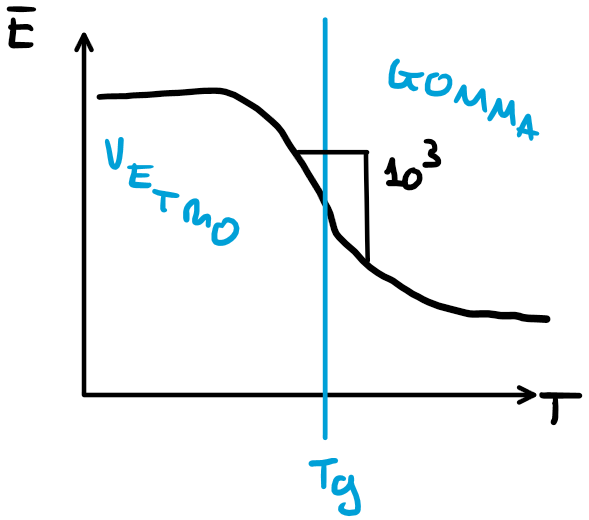
\includegraphics[width = \textwidth]{gfx/Tg}
\caption{Comportamento termico di un materiale amorfo}
\label{fig:Tg}
\end{figure}


Nella realtà, la transizione vetrosa avviene all'interno di un determinato range di temperature. Per convenzione viene fissato la temperatura intermedia a tale range.
A livello microstrutturale non c'è un vero e proprio cambio di struttura nel materiale perché il materiale amorfo era e amorfo rimane.

\begin{figure}
\centering
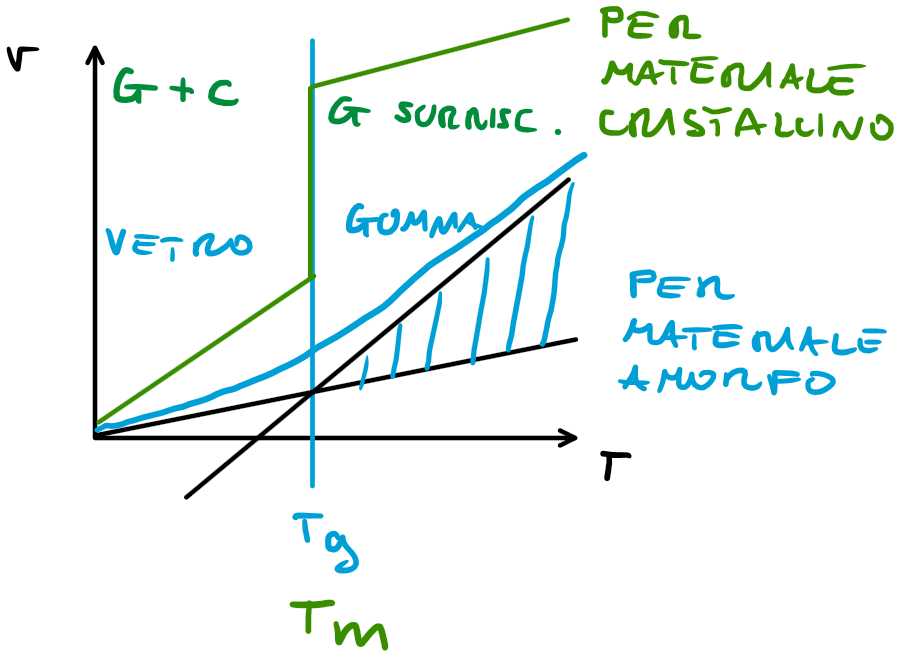
\includegraphics[width = \textwidth]{gfx/VolSpec}
\caption{In termini di volume specifico si vedono in comportamenti per un materiale amorfo e uno semicristallino}
\label{fig:VolSpec}
\end{figure}

Il grafico mostrato in figura \ref{fig:VolSpec}, presenta la variazione del volume specifico in funzione della temperatura sia per un materiale amorfo che per un materiale semi cristallino.
Ciò che accade è che al passaggio attraverso la temperatura di transizione vetrosa $T_g$ aumenta lo spazio libero tra una molecola e l'altra. Determinando, così, una maggiore capacità delle molecole di vibrare attorno ad un punto di equilibrio. Ciò determina anche la repentina diminuzione del modulo elastico. 
Modificando la pressione esterna il comportamento viene traslato verso temperature maggiori, questo perché la pressione limita la vibrazione delle molecole quindi serve più energia per poter ottenere lo stesso comportamento. 

\begin{quote}
\emph{Per un materiale semicristallino?}
\end{quote}


\begin{figure}
\centering
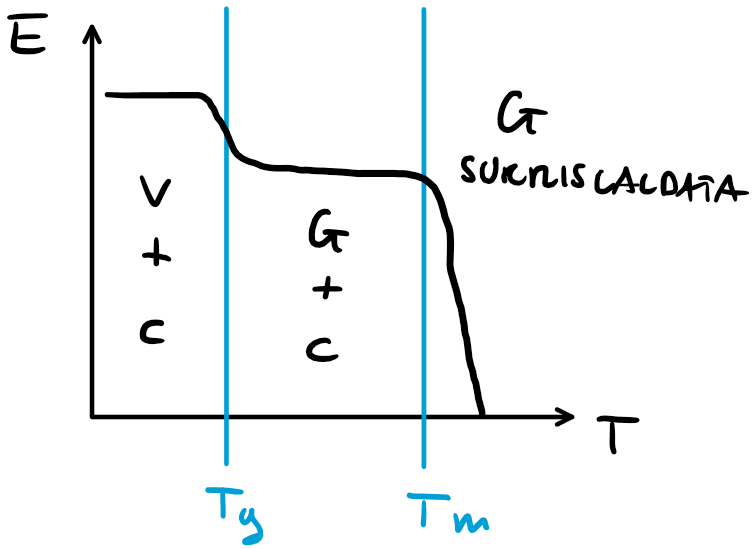
\includegraphics[width = \textwidth]{gfx/TgTm}
\caption{Comportamento termico di un materiale semicristallino}
\label{fig:TgTm}
\end{figure}
Nei materiali semicristallini si ha una vera e propria trasformazione di fase in questo caso si ha una temperatura specifica di trasformazione.

La temperatura di fusione $T_m$ è un unico valore per cui il materiale può essere tranquillamente lavorabile. 
A differenza dei materiali amorfi, la transizione tra materiale cristallino e fluido non risente della pressione in quanto i cristalli sono già compatti.
Dunque, non presentano gli stessi fenomeni evidenziati precedentemente.
 
Per gli amorfi si preferisce oltrepassare il plateau di stato di gomma e avere un materiale molto fluido.
I materiali amorfi vengono utilizzati sempre allo stato vetroso mai gommoso. Sono, tendenzialmente, rigidi e abbastanza resistenti ma fragili. La gomma invece è tendenzialmente duttile e lavorabile.
I materiali cristallini, invece, se utilizzati sotto la temperatura di transizione vetrosa $T_g$ sarebbero materiali eccessivamente fragili. Risulta più conveniente usare all'interno della temperatura di transazione vetrosa e quella di fusione $T_g < T < T_m$. Si ha una gomma rinforzata da cristalli la parte amorfa conferisce tenacità, mentre i cristalli le proprietà meccaniche. 

In generale le plastiche trasparenti sono sempre allo stato vetroso, infatti sono amorfe e di conseguenza fragili. Fa eccezione il \ac{PC} che è a morfo ma non è fragile.
Gli elastomeri sono delle gomme reticolate, per cui conservano le loro proprietà per un buon tratto oltre la temperatura di fusione per via della reticolazione quindi non fondono.

\section{Fattori che influenzano la transizione}
La transizione vetrosa è influenzata da:
\begin{itemize}
\item Mobilità della catena principale,
\item Sostituenti laterali: ingombro e mobilità propria,
\item Legami intermolecolare,
\item Peso molecolare.
\end{itemize}

\paragraph{Mobilità della catena principale}
La transizione vetrosa dipende dalla vibrazione delle molecole attorno alla loro posizione di equilibrio: dunque per catene molto mobili si ha una temperatura di transizione vetrosa più bassa.
Per esempio il \ac{PE} ha una transizione vetrosa a $-100\unit{\celsius}$, decisamente bassa.   
Incrementando la rigidezza della catena polimerica la temperatura di transizione vetrosa aumenta.
Altri materiali:
\begin{itemize}
\item il \ac{PET} ha $T_g = 60\unit{\celsius}$,
\item il \ac{PC} ha $T_g = 120\unit{\celsius}$.
\end{itemize}

\begin{quote}
\emph{Come mai il \ac{PET} lo usiamo a temperatura ambiente anche se risulterebbe vetroso?}
\end{quote}
In questo caso è molto importante il fattore acqua contenuta nell'umidità ambientale.
Tale comportamento, figura \ref{fig:Umidita}, è dovuto ai legami intermolecolari deboli tra le varie catene in cui l'acqua si va ad inserire in mezzo ai legami intermolecolari realizzando una specie di "lubrificazione" tra le molecole. Viene detto \textbf{effetto plastificante}. L'acqua plastifica il polimero, di fatto spezza i legami intermolecolari.
Diminuendo il numero di legami intermolecolari ancora in atto si va a diminuire la temperatura di transizione vetrosa permettendo alle molecole di essere libere a minore energia. 

\begin{figure}
\centering
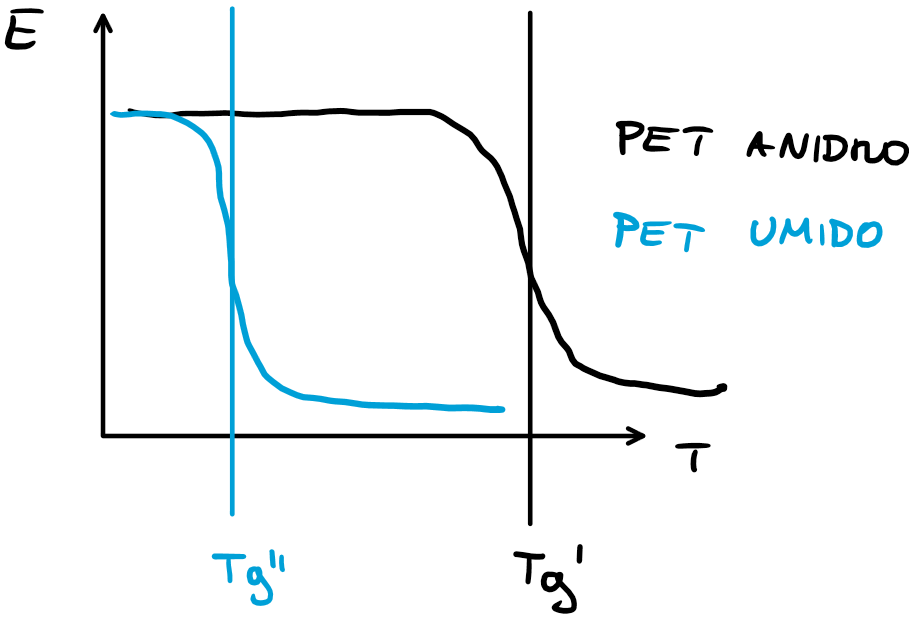
\includegraphics[width = \textwidth]{gfx/Umidita}
\caption{Effetto di abbassamento della transizione per via dell'umidità}
\label{fig:Umidita}
\end{figure}

\paragraph{Sostituenti laterali}
Un sostituente particolarmente ingombrante porta un incremento notevole della $T_g$. Se, per esempio, consideriamo un anello benzenico la temperatura viene aumentata da $-100\unit{\celsius}$ del \ac{PP} a $100\unit{\celsius}$ del \ac{PS}. Mostrati in figura \ref{fig:ConfPPPS}.

\begin{figure}
\centering
\subfloat[][\emph{}\label{fig:PP}]
{%
\begin{minipage}[b]{0.4\textwidth}
\setchemfig{atom sep = 2em}
\schemestart
\chemname{\chemfig{\vphantom{C}-[@{op,.5}]C(-[2]CH_3)(-[6]H)-C(-[2]H)(-[6]H)-[@{cl,.5}]}}{Polipropilene}
\polymerdelim[delimiters ={[]}, indice = n]{op}{cl}
\schemestop
\end{minipage}%
}\quad
\subfloat[][\emph{}\label{fig:PS}]
{%
\begin{minipage}[b]{0.4\textwidth}
\setchemfig{atom sep = 2em}
\schemestart
\chemname{\chemfig{\vphantom{C}-[@{op,.5}]C(-[2]**6(------))(-[6]H)-C(-[2]H)(-[6]H)-[@{cl,.5}]}}{Polistirene}
\polymerdelim[delimiters ={[]}, indice = n]{op}{cl}
\schemestop
\end{minipage}%
}
\caption{Confronto tra i monomeri di polipropilene e polistirene}
\label{fig:ConfPPPS}
\end{figure}

Si può osservare che pur aumentando l'ingombro, se la catena sostituente è molto mobile allora gli effetti si sovrappongono. Il punto è che la mobilità crea molto più volume libero. Dunque l'effetto diventa contrario rispetto a mettere un semplice sostituente. Questo perché bisogna considerare sia il fattore di ingombro che il fattore di mobilità del sostituente in cui la mobilità del sostituente gioca un ruolo più importante.

\paragraph{Legami intermolecolari}
I legami intermolecolari più aumentano in termini di forza e frequenza più la temperatura di transizione vetrosa $T_g$ aumenterà.
Ad esempio il \ac{PVC}, questo genera dei legami intermolecolari più forti. Infatti ha una transizione vetrosa più alta rispetto al polipropilene nonostante siano entrambi materiali vinilici. 

\paragraph{Peso molecolare}
Come era stato anticipato precedentemente, il peso molecolare influisce molto sulla temperatura di transizione vetrosa. Infatti molecole ad alto grado di polimerizzazione avranno sicuramente un peso molecolare più alto ma necessitano di maggiore energia cinetica per potersi muovere.
Siccome necessitano di maggiore energia vuol dire che la temperatura di transizione vetrosa verrà spostata verso valori più alti rispetto a molecole che avendo un grado di polimerizzazione più basso necessiteranno di minore energia per agitarsi.
Risulta essere tutta una questione cinetica.

%************************************************
\chapter{Viscoelasticità}\label{ch:viscoelasticità}
%************************************************
Si tratta della caratterizzazione del comportamento meccanico delle plastiche allo stato solido.

Ipotizzando un materiale solido di cui non si conoscono le caratteristiche meccaniche, la prima prova che si fa è la prova di trazione: si tira e si vede cosa succede.

\begin{quote}
\emph{Si, ma\dots \dots non funziona come per i metalli}
\end{quote}
Infatti si presenta uno sforzo dipendente, si dal carico, anche dalla velocità di deformazione.
In generale, i materiali plastici hanno una forte \textbf{sensibilità alla velocità di deformazione}.
Non è l'unica deviazione dal comportamento dai solidi metallici.

Se un materiale è elastico, allora determinato il modulo elastico, o modulo di Young, si conosce il materiale.
Per le plastiche vale diversamente: se il materiale è completamente amorfo, allora effettivamente l'analisi del modulo elastico è molto significativa per il materiale. Questo però è un caso limite, da non prendere come regola generale.
Dunque, questo tipo di prova non è significativa per i materiali polimerici.

Si preferisce caratterizzarli in altro modo:
\begin{equation}
\sigma = \sigma(\epsilon,\dot{\epsilon})
\end{equation}
ovvero lo sforzo non è determinato solo dalla deformazione ma anche dalla \textbf{velocità di deformazione}.

Allora per caratterizzare il materiale è opportuno misurare proprio le deviazione dal comportamento elastico:
\begin{itemize}
\item Scorrimento viscoso \textbf{Creep},
\item Rilassamento degli sforzi.
\end{itemize}

\paragraph{Rilassamento degli sforzi}
Viene imposta una deformazione costante nel tempo.
Va ricordato che:
\begin{equation}
\epsilon = \frac{L - L_0}{L_0} \quad	\sigma = e(\dot{\epsilon},t)
\end{equation}
Allora il comportamento che si osserva per tale prova è quello delle figure \ref{fig:RilassamentoE} e \ref{fig:RilassamentoS}.

\begin{figure}
\centering
\subfloat[][\emph{Imposizione della deformazione costante}\label{fig:RilassamentoE}]
{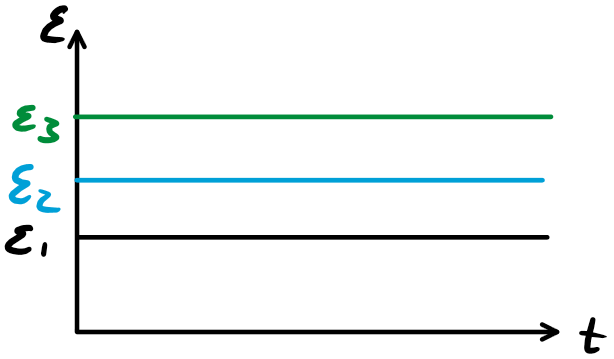
\includegraphics[width = 0.4\textwidth]{gfx/RilassamentoE}}\quad
\subfloat[][\emph{Fenomeno del rilassamento degli sforzi}\label{fig:RilassamentoS}]
{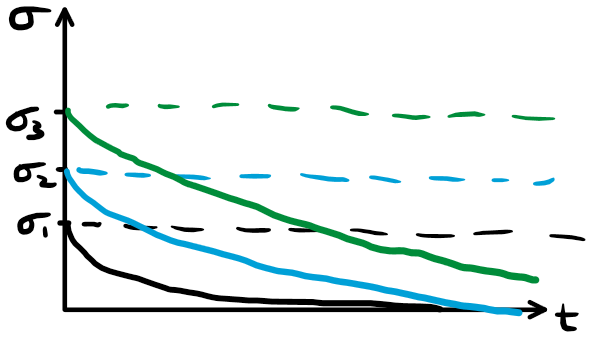
\includegraphics[width = 0.4\textwidth]{gfx/RilassamentoS}}\\
\subfloat[][\emph{Imposizione dello sforzo costante}\label{fig:CreepS}]
{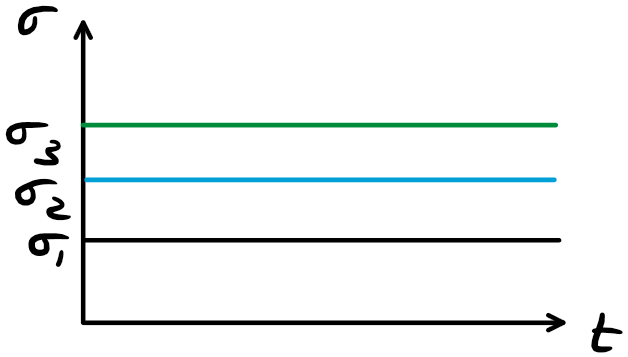
\includegraphics[width = 0.4\textwidth]{gfx/CreepS}}\quad
\subfloat[][\emph{Effetto di \eng{Creep}}\label{fig:CreepE}]
{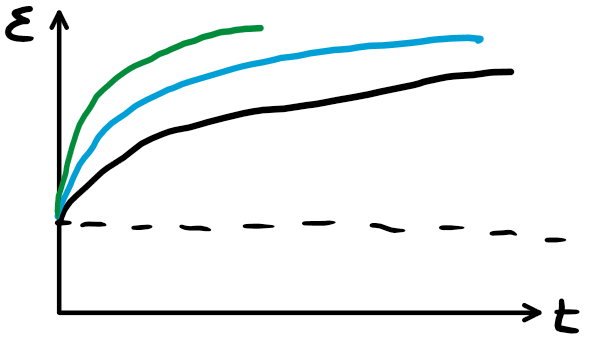
\includegraphics[width = 0.4\textwidth]{gfx/CreepE}}
\end{figure}

\paragraph{Scorrimento viscoso (\eng{Creep})}
Imponendo uno sforzo costante, si osserva l'andamento della deformazione del materiale.

Se la risposta del materiale è lineare, in una delle due variabili, allora la caratterizzazione del materiale può essere più semplice. Sopratutto de il primo degli argomenti di $\bar{\epsilon}$ o $\bar{\sigma}$.

Affinché una funzione sia lineare deve soddisfare entrambe le seguenti:
\begin{align}
f(k*x) &= kf(x) :=\textup{Condizione di funzione omogenea}\\
f(x_1 + x_2) &= f(x_1) + f(x_2) :=\textup{Principio di sovrapposizone degli effetti}
\end{align}